\let\negmedspace\undefined
\let\negthickspace\undefined
\documentclass[journal]{IEEEtran}
\usepackage[a5paper, margin=10mm, onecolumn]{geometry}
%\usepackage{lmodern} % Ensure lmodern is loaded for pdflatex
\usepackage{tfrupee} % Include tfrupee package

\setlength{\headheight}{1cm} % Set the height of the header box
\setlength{\headsep}{0mm}     % Set the distance between the header box and the top of the text

\usepackage{gvv-book}
\usepackage{gvv}
\usepackage{cite}
\usepackage{amsmath,amssymb,amsfonts,amsthm}
\usepackage{algorithmic}
\usepackage{graphicx}
\usepackage{textcomp}
\usepackage{xcolor}
\usepackage{txfonts}
\usepackage{listings}
\usepackage{enumitem}
\usepackage{mathtools}
\usepackage{gensymb}
\usepackage{comment}
\usepackage[breaklinks=true]{hyperref}
\usepackage{tkz-euclide} 
\usepackage{listings}
% \usepackage{gvv}                                        
\def\inputGnumericTable{}                                 
\usepackage[latin1]{inputenc}                                
\usepackage{color}                                            
\usepackage{array}                                            
\usepackage{longtable}                                       
\usepackage{calc}                                             
\usepackage{multirow}                                         
\usepackage{hhline}                                           
\usepackage{ifthen}                                           
\usepackage{lscape}
\usepackage{circuitikz}
\tikzstyle{block} = [rectangle, draw, fill=blue!20, 
    text width=4em, text centered, rounded corners, minimum height=3em]
\tikzstyle{sum} = [draw, fill=blue!10, circle, minimum size=1cm, node distance=1.5cm]
\tikzstyle{input} = [coordinate]
\tikzstyle{output} = [coordinate]

\begin{document}


\bibliographystyle{IEEEtran}
\vspace{3cm}

\title{2.10.79}
\author{EE25BTECH11051 - Shreyas Goud Burra}
\maketitle
{\let\newpage\relax\maketitle}

\renewcommand{\thefigure}{\theenumi}
\renewcommand{\thetable}{\theenumi}
\setlength{\intextsep}{10pt}


\numberwithin{equation}{enumi}
\numberwithin{figure}{enumi}
\renewcommand{\thetable}{\theenumi}

\textbf{Question}\\
In a triangle $PQR$, let\\
$$\textbf{a}=\vec{QR},\, \textbf{b}=\vec{RP},\, \textbf{c}=\vec{PQ}$$
det \textbf{a} = 3,  det \textbf{b} = 4, and

$$\frac{\textbf{a}.(\textbf{c}-\textbf{b})}{\textbf{c}.(\textbf{a}-\textbf{b})}=\frac{\lvert \textbf{a}\rvert}{\lvert \textbf{a}\rvert+\lvert \textbf{b} \rvert}$$

then the value of $\lvert \textbf{a} \times \textbf{b} \rvert$ is \rule{1.5cm}{0.5mm}

\solution\\

Let us find the solution theoretically first and then verify it computationally.\\
It is given that \textbf{a}, \textbf{b} and \textbf{c} are the sides of a triangle. This implies

\begin{align}
    \textbf{a}+\textbf{b}+\textbf{c} = \textbf{QR}+\textbf{RP}+\textbf{PQ} = 0
    \label{0.1}
\end{align}

It is also given that,
\begin{align}
    \lvert \textbf{a} \rvert=3\text{ and }\lvert \textbf{b} \rvert = 4
    \label{0.2}
\end{align}

Let the given equation,
\begin{align}
    \frac{\textbf{a}.(\textbf{c}-\textbf{b})}{\textbf{c}.(\textbf{a}-\textbf{b})}=\frac{\norm{\textbf{a}}}{\norm{\textbf{a}}+\norm{\textbf{b}}}
    \label{0.3}
\end{align}

This gives,

\begin{align}
    \frac{\textbf{a}.(\textbf{c}-\textbf{b})}{\textbf{c}.(\textbf{a}-\textbf{b})}=\frac{3}{7}
    \label{0.4}
\end{align}

On further simplifying this gives us,

\begin{align}
    7(\textbf{a}^{\text{T}}\textbf{c}-\textbf{a}^{\text{T}}\textbf{b})=3(\textbf{c}^{\text{T}}\textbf{a}-\textbf{c}^{\text{T}}\textbf{b})
    \label{0.5}
\end{align}

\begin{align}
    4\textbf{a}^{\text{T}}\textbf{c}-7\textbf{a}^{\text{T}}\textbf{b}+3\textbf{c}^{\text{T}}\textbf{b}=0
    \label{0.6}
\end{align}

On multiplying $\textbf{a}^{\textbf{T}}$ on both sides of \ref{0.1}

\begin{align}
    \textbf{a}^{\text{T}}\textbf{a}+\textbf{a}^{\text{T}}\textbf{b}+\textbf{a}^{\text{T}}\textbf{c}=0 \implies \textbf{a}^{\text{T}}\textbf{b}+\textbf{a}^{\text{T}}\textbf{c}=-9
    \label{0.7}
\end{align}

On multiplying $\textbf{b}^{\textbf{T}}$ on both sides of \ref{0.1}

\begin{align}
    \textbf{b}^{\text{T}}\textbf{a}+\textbf{b}^{\text{T}}\textbf{b}+\textbf{b}^{\text{T}}\textbf{c}=0 \implies \textbf{b}^{\text{T}}\textbf{a}+\textbf{b}^{\text{T}}\textbf{c}=-16
    \label{0.8}
\end{align}

On solving the equations \ref{0.6}, \ref{0.7} and \ref{0.8}

\begin{align}
    \myvec{-7 & 3 & 4 \\ 1 & 0 & 1\\1 & 1 & 0} \myvec{\textbf{a}^\text{T}\textbf{b}\\\textbf{b}^\text{T}\textbf{c}\\\textbf{c}^\text{T}\textbf{a}\\}=\myvec{0\\-9\\-16}
    \label{0.9}
\end{align}

On using Gauss Jordan method to solve this
\begin{align}
    \myvec{\textbf{a}^\text{T}\textbf{b}\\\textbf{b}^\text{T}\textbf{c}\\\textbf{c}^\text{T}\textbf{a}\\}=\myvec{-7 & 3 & 4 &| & 0\\1& 0 & 1 & | &-9\\1&1&0&|&-16}
    \label{0.10}
\end{align}

On doing $R_1\rightarrow R_1+8R_2$ and $R_3\rightarrow R_3-R_2$

\begin{align}
    \myvec{\textbf{a}^\text{T}\textbf{b}\\\textbf{b}^\text{T}\textbf{c}\\\textbf{c}^\text{T}\textbf{a}\\}=\myvec{1 & 3 & 12 &| & -72\\1& 0 & 1 & | &-9\\0&1&-1&|&-7}
    \label{0.11}
\end{align}

On doing $R_2\rightarrow R_2-R_1$

\begin{align}
    \myvec{\textbf{a}^\text{T}\textbf{b}\\\textbf{b}^\text{T}\textbf{c}\\\textbf{c}^\text{T}\textbf{a}\\}=\myvec{1 & 3 & 12 &| & -72\\0& -3 & -11 & | &63\\0&1&-1&|&-7}
    \label{0.12}
\end{align}

On doing $R_1 \rightarrow R_1 + R_2$ and $R_3 \rightarrow R_3+\frac{1}{3}R_2$

\begin{align}
    \myvec{\textbf{a}^\text{T}\textbf{b}\\\textbf{b}^\text{T}\textbf{c}\\\textbf{c}^\text{T}\textbf{a}\\}=\myvec{1 & 0 & 1 &| & -9\\0& -3 & -11 & | &63\\0&0&-\frac{14}{3}&|&14}
    \label{0.13}
\end{align}

On doing $R_1\rightarrow R_1+\frac{3}{14}R_3$ and $R_2\rightarrow R_2-\frac{33}{14}R_3$

\begin{align}
    \myvec{\textbf{a}^\text{T}\textbf{b}\\\textbf{b}^\text{T}\textbf{c}\\\textbf{c}^\text{T}\textbf{a}\\}=\myvec{1 & 0 & 0 &| & -6\\0& -3 & 0 & | &30\\0&0&-\frac{14}{3}&|&14}
    \label{0.14}
\end{align}

From this, we get,

\begin{align}
    \textbf{a}^\text{T}\textbf{b}=-6
    \label{0.15}
\end{align}

From the definition of cross product, and from \ref{0.15} we get,

\begin{align}
    \norm{\textbf{a} \times \textbf{b}}^2 = \norm{\textbf{a}}^2 \norm{\textbf{b}}^2-(\textbf{a}^\text{T}\textbf{b})^2 
    \implies \norm{\textbf{a} \times \textbf{b}}^2 = 4^2 . 3^2 -(-6)^2
    \label{0.16}
\end{align}

The final answer,

\begin{align}
    \norm{\textbf{a} \times \textbf{b}} = 6\sqrt{3}
\end{align}

The plot for the given question is given below,

\begin{figure}[H]
    \centering
    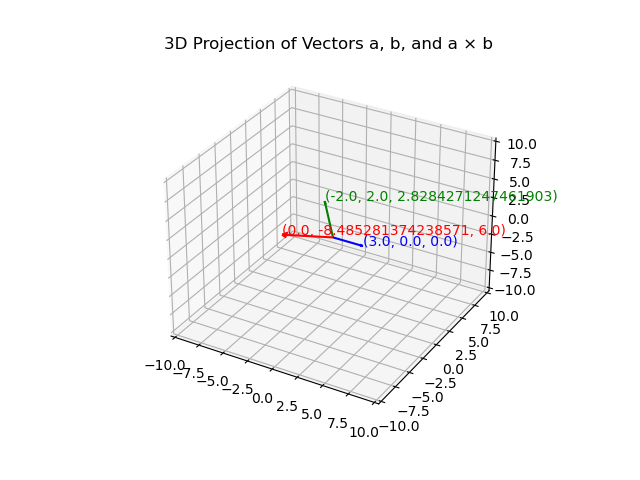
\includegraphics[width=0.8\columnwidth]{figs/fig1.png}
    \caption{3D Plot}
    \label{3D Plot}
\end{figure}

\end{document}
